\documentclass[11.5pt]{sig-alternate} % sets document style to sig-alternate
% packages
% typesetting
%\usepackage{dirtytalk} % typset quotations easier (\say{stuff})
\usepackage{hanging} % hanging paragraphs
\usepackage[defaultlines=3,all]{nowidow} % avoid widows
\usepackage[pdfpagelabels=false]{hyperref} % produce hypertext links, includes backref and nameref
\usepackage{xurl} % defines url linebreaks, loads url package
\usepackage{microtype}
%\usepackage[super]{nth} % easily create superscript ordinal numbers with \nth{x}\
\usepackage{enumitem}
\usepackage{textgreek}
% layout
\usepackage{enumitem} % control layout of itemize, enumerate, description
\usepackage{fancyhdr} % control page headers and footers
\usepackage{float} % improved interface for floating objects
%\usepackage{multicol} % intermix single and multiple column pages
% language
\usepackage[utf8]{inputenc} % accept different input encodings
\usepackage[english]{babel} % multilanguage support
% misc
\usepackage{graphicx} % builds upon graphics package, \includegraphics
%\usepackage{lastpage} % reference number of pages
%\usepackage{comment} % exclude portions of text (?)
\usepackage{xcolor} % color extensions
\usepackage[backend=biber, style=apa]{biblatex} % sophisticated bibliographies % necessary for HTML to display author info and date on abstract page
\usepackage{csquotes} % advanced quotations, makes biblatex happy
\usepackage{authblk} % support for footnote style author/affiliation
% tables and figures
\usepackage{tabularray}
%\usepackage{array} % extend array and tabular environments
\usepackage{caption} % customize captions in figures and tables (rotating captions, sideways captions, etc)
%\usepackage{cuted} % allow mixing of \onecolumn and \twocolumn on same page
\usepackage{multirow} % create tabular cells spanning multiple rows
%\usepackage{subfigure} % deprecated, support for manipulation of small figures
%\usepackage{tabularx} % extension of tabular with column designator "x", creates paragraph-like column whose width automatically expands
%\usepackage{wrapfig} % allows figures or tables to have text wrapped around them
%\usepackage{booktabs} % better rules
% dummy text
%\usepackage{blindtext} % blind text dummy text
%\usepackage{kantlipsum} % Kant style dummy text
\usepackage{lipsum} %lorem ipsum dummy text
% other helpful packages may be booktabs, longtable, longtabu, microtype

\pagestyle{fancy} % sets pagestyle to fancy for fancy headers and footers

% header and footer
% modern way to set header image
\renewcommand{\headrulewidth}{0pt} % defines thickness of line under header
\renewcommand{\footrulewidth}{0pt} % defines thickness of line above header
\setlength\headheight{80.0pt} % sets height between top margin and header image, effectively moves page contents down
\addtolength{\textheight}{-80.0pt} % seems to affect the lower height. maybe only works properly if footer numbers enabled?
\fancyhf{}
\fancyhead[CE, CO]{
\includegraphics[width=\textwidth]{headerImage.png}}
% footer
%\fancyfoot[LE,LO]{Article Title Here \\ DOI: }% left footer article title and doi
%\fancyfoot[CE,CO]{{}} % center footer empty
%\fancyfoot[RE,RO]{\thepage} % right footer page numbers
%\pagenumbering{arabic} % arabic (1, 2, 3) numbering in footer

\hypersetup{colorlinks=true,urlcolor=blue} % sets link color to blue
\urlstyle{same} % sets url typeface to same as rest of text

% set caption and figure to italics, label bold, left align captions, does not transfer to HTML
\DeclareCaptionFormat{custom}
{
    \textbf{\textit{\large #1#2}}\textit{\large #3} % #1 is the "Table 1" or "Figure 1" part, #2 is the separator (":"), #3 is the caption
}
\captionsetup{format=custom}
\captionsetup{justification = raggedright, singlelinecheck = false}

%this next bit is confusing, but essentially changes the width of the abstract. Seems to have been copied from this https://tex.stackexchange.com/questions/151583/how-to-adjust-the-width-of-abstract
\let\oldabstract\abstract
\let\oldendabstract\endabstract
\makeatletter %changes @ catcode to enable modification (in parsep)
\renewenvironment{abstract} %alters the abstract environment
{\renewenvironment{quotation}%
               {\list{}{\addtolength{\leftmargin}{1em} % change this value to add or remove length to the the default ?
                        \listparindent 1.5em%
                        \itemindent    \listparindent%
                        \rightmargin   \leftmargin%
                        \parsep        \z@ \@plus\p@}%
                \item\relax}%
               {\endlist}%
\oldabstract}
{\oldendabstract}
\makeatother %changes @ catcode to disable modification

\begin{document}

\title{Visualization without Vision – How Blind and Visually Impaired Students and Researchers Engage with Molecular Structures}

\author[1]{\large \color{blue}Croix J. Laconsay}
\author[1]{\large \color{blue}Henry B. Wedler}
\author[1]{\large \color{blue}Dean J. Tantillo}

\affil[1]{Department of Chemistry University of California-Davis}

\toappear{}
%% ABSTRACT
\maketitle
\begin{@twocolumnfalse} 
\begin{abstract}
\item 
\textit {This article examines the tools and techniques currently available that enable blind and visually impaired (BVI) individuals to visualize three-dimensional objects used in learning chemistry concepts. How BVI individuals engage with and visualize molecular structure is discussed and recent tactile (or haptic) and auditory methods for visualization of various chemistry concepts are summarized. Remaining challenges for chemistry education researchers are described with the aim of highlighting the potential value of educational research in further enabling BVI students to pursue careers in science, technology, engineering, and mathematics (STEM) fields.}
\\ \\
Keywords: chemistry, blind/low vision, accessibility, 3D printing, molecular structure
\end{abstract}
\end{@twocolumnfalse}

%% AUTHOR INFORMATION

\textbf{*Corresponding Author, Dean J. Tantillo}\\
\href{mailto:djtantillo@ucdavis.edu}{djtantillo@ucdavis.edu} \\
\textit{Submitted  March 1, 2020}\\
\textit{Accepted April14, 2020} \\
\textit{Published online July 23, 2020} \\
\textit{DOI: 10.14448/jsesd.12.0012} \\
\pagebreak
\clearpage

\begin{large}
\section*{INTRODUCTION}

Chemistry is, inherently, a visual science. Chem\-ists play in both the micro- and macroscopic worlds of molecules, and communication of connections between concepts in both realms is facilitated by visual representations (Grosholz and Hoffmann, 2000; Hoffmann, 2007; Hoffmann and Laszlo, 1991). Students of this science rely heavily on 2-dimensional (2D) and 3-dimensional (3D) visualizations of molecular structures when learning chemical concepts and solving chemical problems (Mathewson, 1999). Readers of this article are referred to Wu and Shah’s review for a comprehensive account on visuospatial thinking in chemistry learning (Wu \& Shah, 2004). Visualization, however, should not be equated with having vision. “There is much more to the visualization than the sense of vision, and impaired vision does not necessarily preclude our faculties to visualize.” (Figueiras and Arcavi, 2015). 

The visual aspects of chemistry can deter blind and visually impaired (BVI) students from entering the field. Moreover, literature on enabling BVI students in chemistry is generally lacking. Several recent efforts to make chemistry more accessible to BVI students have been described in the chemistry education literature: in particular, methodologies for facilitating engagement of BVI students with molecular structures — the basis of this perspective article. 

A note on what this article is and is not. This perspective is not an exhaustive review on tools that enable BVI students in all of chemistry, as there are many aspects of the subject that are beyond the scope of this article. For instance, much of chemistry involves \textit{symbolic} representation as opposed to \textit{structural} representation. Teke and Sozbilir recently addressed problems of symbolic representation that blind students experience when learning chemistry (Teke \& Sozbilir, 2019). There is substantial literature aimed at enabling BVI individuals to participate in other aspects of chemistry not explicitly related to chemical (molecular) structure and other science, technology, engineering, and mathematics (STEM) fields; curious readers are directed to the following recent references for examples: (a) exploring chemistry topics in the formal classroom (Smith, 1981; Stender et al., 2016; Tombaugh, 1981) and laboratory settings (Andersen, 1982; Bromfield-Lee \& Oliver-Hoyo, 2007; Flair \& Setzer, 1990; JCE staff, 2000; Neppel, Oliver-Hoyo, Queen, \& Reed, 2005; Supalo, Mallouk, Rankel, Amorosi, \& Graybill, 2008; J. T. Wood \& Eddy, 1996), (b) exploring chemistry topics in informal teaching settings (Kumar \textit{et al}., 2018), (c) solving puzzles (Cady, 2012) and using interlocking toy building blocks, like Legos, to learn chemistry (Campbell, Miller, Bannon, \& Obermaier, 2011; Cloonan, Nichol, \& Hutchinson, 2011; Geyer, 2017; Melaku, Schreck, Griffin, \& Dabke, 2016; Ruddick \& Parrill, 2012; Witzel, 2002), (d) three-dimensionally printed puzzle pieces for representing elements, ions, compounds, or a chemical equations (Singhal \& Balaji, 2019), (e) a musical electrochemical cell (Cady, 2014), (f) development of a BVI-accessible thermometer (Vitoriano \textit{et al}., 2016), (g) science enrichment activities at National Federation of the Blind Youth Slams (Supalo \textit{et al}., 2014) and science camps (Supalo, \textit{et al}., 2014; Wedler \textit{et al}., 2014), (h) approaches aimed at secondary school education (Supalo \textit{et al}., 2016). For an excellent case study of a student with blindness successfully completing a chemistry laboratory course, see the recent report in this very \textit{Journal} (Michael \& Wohlers, 2019). 

According to the Individuals with Disabilities Education Act of 2004 (IDEA) definition, a visual impairment is, “an impairment in vision that, even with correction, adversely affects a child’s educational performance. The term includes both partial sight and blindness” (Individuals with Disabilities Education Act, 2004). Individuals with visual impairments are not necessarily legally or congenitally blind. Many individuals with visual impairments still have some sight, which affects how they engage with different forms of representation. The United States BVI population faces a significant unemployment rate, estimated to be as high as 72\% as of 2015 (National Federation of the Blind Statistical Facts about Blindness in the United States, \url{https://nfb.org/blindness-statistics}, accessed 2 November 2018). Of the employed population of individuals with any disability, less than 4.5\% work in STEM disciplines (Table 3. Employed persons by disability status, occupation, and sex, 2018 annual averages; sum of "computer and mathematical," "architecture and engineering" and "life, physical, and social science" occupations and, therefore, likely an overestimate, since architecture and social science are generally not considered part of STEM), a percentage that has recently decreased since we last reported the statistic in 2014 (Statistics, Survey, States, \& Policy, 2018; Wedler et al., 2014). To our knowledge, statistics on the fraction of this group working in chemistry are not available, but given that the percentage of the total US population estimated to have a visual impairment is approximately 2\% (National Federation of the Blind Statistical Facts about Blindness in the United States, \url{https://nfb.org/blindness-statistics}, accessed 2 November 2018), we expect that BVI individuals are underrepresented in chemistry. 

Students with blindness or low vision experience and engage the world differently than their sighted peers, but this does not imply that BVI individuals cannot succeed in STEM careers. There are many examples of successful scientists with limited to no vision. These include: Mona Minkara at Northeastern University (chemist), Geerat J. Vermey at UC Davis (evolutionary biologist and paleontologist), Amy Bower at Woods Hole Oceanographic Institution (oceanographer), David Mehringer at the National Radio Astronomy Observatory (software developer and astronomer), Wanda Díaz-Merced at the South African Astronomical Observatory (astronomer), Judith Summers-Gates of the U.S. Food and Drug Administration (chemist), David Wohlers of Truman State University (chemist), and Peter Torpey of the “Eyes On Success” podcast (previously at Xerox, now podcast host).

\subsection*{How do blind and visually impaired students engage with molecular structure?}

What is it we mean by molecular or chemical structure? By molecular or chemical structure, we mean collections of atoms connected by bonds to form a molecule. Chemical or molecular structures have defined spatial and symmetry properties that can be used to explain said structures to BVI chemists, e.g., distances between nuclei, angles defined by the positions of three nuclei, molecular point group symmetry. The geometric properties of a molecule have many implications for chemistry research and education, e.g., predicting sites of chemical reactivity in a molecule, predicting how a small molecule (such as a drug) binds to a protein, predicting spectral properties. These types of predictions rely on practitioners being comfortable with patterns that are defined by similarities in molecular structures.

There is compelling evidence that BVI and non-BVI individuals have equal ability to process spatial information (Zimler \& Keenan, 1983). Moreover, like their sighted peers, BVI individuals possess similar, and arguably superior, cognitive and perceptual abilities regarding analyzing and exploring tactile pictures (D’Angiulli, Kennedy, \& Heller, 1998). For a perspective on how students with blindness or low vision process and learn science concepts, readers are referred to the work of Jones and Broadwell (Jones and Broadwell, 2008).

A co-author of this review, HBW, completely blind since birth, received his Ph.D. in organic chemistry in 2016. Henry, or “Hoby”, explains that,

\begin{quote}
    I use the same skills to visualize molecular structures as I have used since day 1 for my survival as a blind traveler. I cannot see maps, streets, etc., so I must visualize everything. When I ponder the route from the chemistry building to the nearest bus stop in my mind, for instance, it feels the same as pondering a complex molecular structure and determining where atoms are relative to one another. The distance between points doesn’t matter when I visualize a physical space or chemical structure. If I’m visualizing a space, I think in meters and kilometers. When I think about chemical structures, I think precisely the same way but in angstroms and nanometers. 
\end{quote}

Jones \textit{et al}. supports this notion: visually impaired students were more accurate with measurements at very large (e.g., distance from earth to mars) and very small (e.g., bond length of C–H bond) scales compared to their normal sighted peers (G. Jones, Taylor, \& Broadwell, 2009). Hoby continues by explaining that,  

\begin{quote}
    I often have an easier time with reaction mechanisms than some sighted peers because I can place structures in my mind and understand actual distances between atoms. Two atoms that look extremely far apart from each other may be very close together in space and my 3D understanding of molecular structure helps me here. Ultimately, thinking about how to get around a college campus or familiar town is not very different than thinking about solving a complicated reaction mechanism. Thinking about the steps that I need to take on a route I am traveling is analogous to solving an organic synthesis problem. Often when figuring out how to travel a multi-city, multi-step route, I look at the route holistically and break it up “retrosynthetically” much the same way that I begin to solve synthesis problems.
\end{quote}

For another perspective from a blind chemist on learning chemistry, see the work of Supalo (Supalo, 2005). We also note an excellent article by Mona Minkara, a blind computational chemist, wherein she describes how she implemented methods that enabled her to complete graduate work at the University of Florida (Minkara, Weaver, Gorske, Bowers, \& Merz, 2015). In addition to more articles like the ones mentioned above, we hope to see future basic neuroscience research that elucidates whether the brain processes information about macroscopic and microscopic navigation in a similar manner as described by Hoby. 

\subsection*{Current methods for engaging with molecular structures}

In this section, we summarize some of the non-vision-based methods that enable BVI students and researchers engage with molecular structure. We describe developments in tactile (or touch)-based methods, which have advanced significantly with the incorporation of 3D printing technology. Then we introduce recent advances in utilizing audio (or sound)-based methods for engaging with molecular structures. 

\subsubsection*{Raising the bar with tactile graphics and three-dimensional (3D) printed models}

The use of tactile graphics—in the form of braille, raised lines and surfaces—is one approach for conveying structural information to BVI individuals. Horton \textit{et al}. summarize tactile technology in general available for BVI individuals in a recent review (Horton \textit{et al}., 2017) – we focus our perspective on approaches that have found use in chemistry. The Independent Laboratory Access for the Blind (ILAB), a project by multiple universities and funded by the National Science Foundation, is a good start (\url{http://research.chem.psu.edu/mallouk/ilab/}, accessed 20 February 2020) for readers looking for tactile classroom and laboratory tools that enable BVI students. The ILAB, for example, provides laboratory tools and techniques for BVI students to perform laboratory experiments without sighted assistance. In addition, and in a similar way that ILAB provides BVI-accessible tools for laboratory settings, MOLinsight (Pereira, Aires-De-Sousa, Bonifácio, Mata, \& Lobo, 2011) provides a one-stop-shop for BVI-accessible open-source software resources (\url{http://molinsight.net/}, accessed 3 March 2020) like NavMol and BrailChem. We discuss alternative and more recent methods below. For teaching tools in the organic chemistry classroom, Fernández \textit{et al}. described some of the hands-on activities available to for teaching organic Lewis structures, Newman and Fischer Projections, and resonance (Fernández, Ocampo, Costantino, \& Dop, 2019).

Much of chemistry for sighted students is communication and representation of chemical structure by pen and paper. For BVI individuals, the pen and paper method approach to representing chemical structure is more challenging without a sighted assistant. For more rapid tactile access to visual information, we developed a workflow in which a sighted assistant draws an image and then raises the lines of the figure (Wedler \textit{et al}., 2012). First, the sighted assistant views the figure; the subsequent process works best if the assistant is familiar with the chemistry involved in the image. Then, he/she draws the image on thick, smooth paper, ideally at least three times as large as the image would normally appear in print. Then, the assistant flips the smooth paper over and places it on a soft pad, such as a notebook or rubber mat. The assistant then traces the inverse of the drawn figure with a ballpoint pen, while applying significant pressure with the pen tip. This pressure creates a crease in the paper using the soft pad beneath, embossing the image so that the BVI student can feel the image (not its mirror image) when the paper is flipped over. It is helpful if BVI chemistry students can recognize common upper-case letters tactilely so that braille versions of element symbols are not necessary, but the paper can be brailled using a standard Perkins Brailler (e.g., see \url{https://brailler.perkins.org/}, accessed 2 November 2018). This method is inexpensive and fast with a trained student-assistant pair (Wedler \textit{et al}., 2012). Creative adaptive tools to represent molecular structures—like the use of magnetic letters and numbers on a magnetic board or tactile model kit (Boyd-Kimball, 2012), crayons and mesh, “thermopens”, or standard inkjet on thermal paper raised by a tactile graphic maker to create raised digital images (Harshman, Bretz, \& Yezierski, 2013)—have been implemented in chemistry classrooms as well.

Specifically applicable to organic chemistry, Supalo and Kennedy have summarized commercially available equipment available to turn organic structures into BVI individual accessible structures (Supalo and Kennedy, 2014). ChemDraw’s text-to-speech output, picture in a flash technology, and the Draftsman tactile drawing board (\url{https://www.aph.org/product/draftsman-tactile-drawing-board/}, accessed 17 February, 2020) are all tools that can make organic structures more accessible. 

Three-dimensional (3D) printing has recently become a commonplace and affordable technology. In chemistry classrooms, 3D printing can change how molecular structure is taught (e.g., \url{https://youtu.be/sSAz\_r5gIc4}, accessed 7 November 2018); (Anderson, 2017; Brauner, 2018; Pinger, Geiger, \& Spence, 2019). In recent years, 3D-printed models related to chemistry have been reported: for example, small molecules (Wieren et al., 2017), extended molecular structure representations (Figure 1) (Rossi \textit{et al}., 2015), electron density isosurface models (Grumman \& Carroll, 2019),  solid state crystal structures (Kitson et al., 2014; Stone-Sundberg, Kaminsky, Snyder, \& Moeck, 2015; P. A. Wood et al., 2017) potential energy surfaces (Blauch \& Carroll, 2014; Kaliakin, Zaari, \& Varganov, 2015; Teplukhin \& Babikov, 2015), orbitals (Lolur and Dawes, 2014; Griffith \textit{et al}., 2016; Smiar and Mendez, 2016; Carroll and Blauch, 2018; De Cataldo \textit{et al}., 2018; Robertson and Jorgensen, 2015)), 3D models for teaching symmetry (Casas \& Estop, 2015; Scalfani \& Vaid, 2014), block copolymer nanostructures (Scalfani \textit{et al}., 2015) and models for teaching VSEPR theory (Dean \textit{et al}., 2016). While many structures can be represented using off-the-shelf molecular model kits, these papers highlight structure representations and applications that are enabled by 3D printing.

\begin{figure}[h]
    \centering
    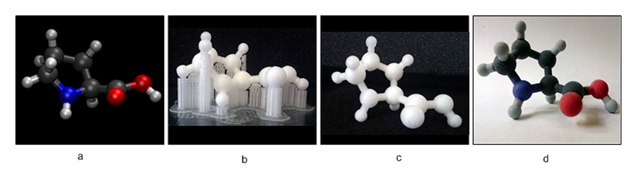
\includegraphics[width=1\linewidth]{fig1.png}
    \caption{Reproduced with permission from Figure 1 of \textit{J. Chem. Educ.} \textbf{2015}, \textit{92}, 1398-1401. Copyright 2015 American Chemical Society.}
\end{figure}

An example of 3D printing increasing accessibility to a traditionally inaccessible (to blind students) area of chemistry is its application to applied computational chemistry. Applied computational chemistry is the use of quantum chemistry calculations to investigate problems in other sub-disciplines of chemistry, e.g., organic chemistry (i.e. applied computational organic chemistry). This approach was used by HBW to allow him to carry out research independently (Wedler et al., 2012). SMILES (Simplified Molecular Input Line Entry Specification) strings (Weininger \textit{et al}., 1989) and Open Babel software (Guha et al., 2006) were used to generate 3D coordinates of complex molecules, since standard molecule-building graphical user interfaces (GUIs) are not accessible to blind individuals. SMILES strings consist of text that encodes connectivity and stereochemical information for organic molecules, and as such can be written by hand. The Open Babel software translates such connectivity and stereochemical information into reasonable atomic coordinates that can then be subject to quantum chemical calculations. The data from these can be analyzed using simple Bash and Perl scripts that extract relevant data from long output files. Readers are referred to Wedler \textit{et al}., 2012 for further details. Subsequent studies (Wedler \textit{et al}., 2015; Wedler, Newman, and Tantillo, 2016) showcase two research projects that were carried out utilizing this methodology.

To increase the information content of 3D-printed molecules, Lounnas \textit{et al}. developed a modified version of AsteriX—web-based software that converts 2D representations of compounds to 3D structures—called AsteriX-BVI. By incorporating textures and braille annotations onto tactile models, different types of atoms and bonds could be distinguished using touch (Lounnas \textit{et al}., 2014); see Figure 2.

\begin{figure}[h]
    \centering
    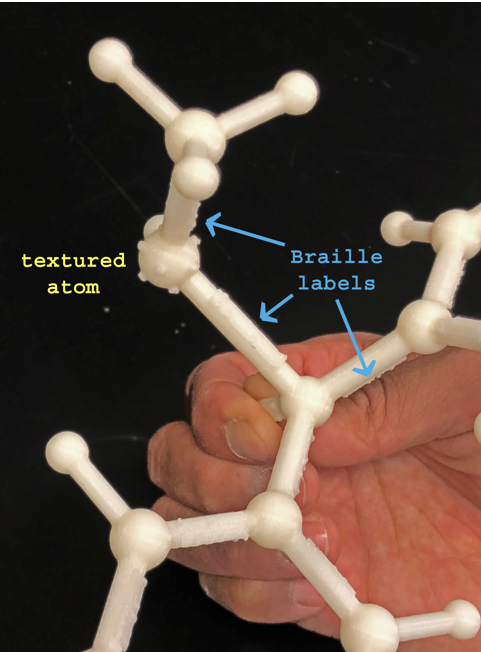
\includegraphics[width=1\linewidth]{fig2.png}
    \caption{Example of a haptic (tactile) model calculated by AsteriX- BVI.}
\end{figure}

\newpage
\subsection*{Tools All Out on the Table, The Periodic Table of the Elements (PTE)}

Other researchers have also tackled aspects of chemistry that are related to molecular structure, such as the periodic table of the elements (PTE). The PTE is a central—visual—tool for understanding and predicting the behavior of chemical elements. As one navigates from element to element, patterns emerge, patterns that chemists use in teaching general chemistry to undergraduates and to inform their research (Scerri, 2007). Melaku \textit{et al}. developed modules involving interlocking toy building blocks like Legos to teach BVI individuals PTE trends—such as atomic radii, ionization energies, electronegativities—and molecular orbitals in homonuclear diatomic molecules (Figure 3) (Melaku et al., 2016).

\begin{figure}[h]
    \centering
    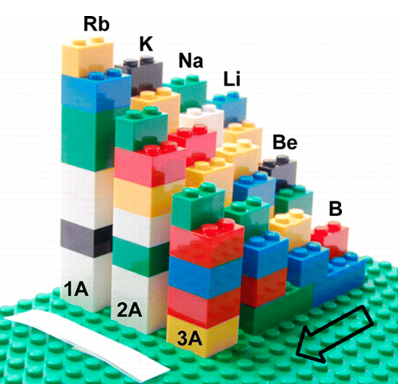
\includegraphics[width=1\linewidth]{fig3.png}
    \caption{Building block modules representing relative atomic and cationic radii of a few elements of Groups 1A, 2A, and 3A. Reproduced with permission from Figure 1 of \textit{J. Chem. Educ.} \textbf{2016}, \textit{93}, 1049-1055. Copyright 2015 American Chemical Society.}
\end{figure}

Another tactile and audio-enhanced PTE (Fantin \textit{et al}., 2016) was developed by Touch Graphics Inc., which utilizes bar code labels on each element square that can be recognized by a Smart Pen. This PTE folds out from four brailled pages containing all elements laid out in standard fashion. Each tactile square lists the element symbol and atomic number in braille. Since braille takes up much more space than print, it would be impossible to include all standard information from a PTE in braille, but users can tap each element of the PTE using a Smart Pen and access relevant information such as atomic mass, melting point, boiling point, electron configuration, etc. in audio format. Roy Alexander also has a tactile PTE called the Element Book (\url{http://www.aaeinfo.us/braille/}, accessed 17 February, 2020). Further developed PTE’s include a 3D-printed PTE with braille lettering (LeSuer, 2019). Classroom activities that engage students with the PTE such as The People Periodic Table activity are also potential tools for enabling BVI students in discussions about PTE trends (Hoffman\& Hennessy, 2018). Mobile tools have been introduced as a way for BVI students to learn about the PTE audibly with their smart phones, such as a QR-coded audio PTE called QR-APTE (Bonifácio, 2012), the Royal Society of Chemistry’s “Elements articles” (\url{https://www.chemistryworld.com/218.subject}, accessed 2 November 2018), and the Elementor Periodic Table App (\url{https://www.perkinselearning.org/accessible-science/activities/elementor-periodic-table-app}, accessed 19 February 2020)—auditory tools in chemistry will be discussed more below. For a discussion on current challenges faced by the chemistry community in fostering learning of the PTE for BVI individuals, including discussions of other accessible PTEs, see the work by Fantin et al. (Fantin \textit{et al}., 2016). 

\subsection*{Sonified chemistry}

In addition to haptic/tactile methods, auditory/aural methods provide another opportunity for conveying information to BVI individuals. When coupled together, haptic and auditory methods have been shown to amplify one’s ability to visualize representations (Grabowski \& Barner, 1998). Early studies aimed at making chemistry more accessible through auditory feedback focused on the teaching laboratory environment, e.g., conductivity and titration experiments (Hiemenz and Pfeiffer, 1972; Ratliff, 1997). We focus here on audio tools for listening to chemical spectra and for reading the chemical literature. 

Traditionally, chemical spectra, used routinely to identify and quantify molecular composition, are also generally presented in visual formats. The inherent complexities of most spectra make “reading” the spectra through touch impractical. Of course, visual spectra are, in fact, just created from numbers, numbers that could be presented in nonvisual formats. For example, Pereira and co-workers have developed a methodology for converting infrared (IR) spectroscopy data into nonspeech audio sound called “sonified infrared spectra (SIRS)” (Pereira \textit{et al}., 2013). All that is needed to use SIRS is experimental IR data and open-source software (JDXview v0.2 and CSV to MIDI converter). Through SIRS, raw IR data (e.g., obtained from spectra from the National Institute of Standards and Technology database) in the form of transmittance is converted to a range of musical instrument frequencies, which correspond to specific absorption peaks. The researcher, who first requires specialized audio training to be able to recognize characteristic functional groups, can then listen to the sound file and analyze the SIRS spectrum. A more recent high-school project based on sonification of IR absorbances to make key chemical vibrations (key wavenumbers on an IR spectrum) into musical notes further advances this concept that chemical spectra can be pushed beyond the visual representation (Garrido et al., 2020). Other examples of sonified chemistry include Bandyopadhyay and Rathod’s application called “Titration ColorCam (TCC)” — a smartphone aid for assisting color-blind and BVI students in titration experiments (Bandyopadhyay and Rathod, 2017). This application exploits a smartphone’s built-in camera function to quantify changes in color during a titration experiment and convert that into audio (beep sounds) and haptic (vibrations) output, thereby allowing a student to determine the end-point of a titration experiment.  

Text-to-speech software enables simple text to be read aloud to BVI individuals but conveying information in figures in chemistry textbooks and research papers in a non-visual format remains a major challenge. In many (most) cases, figure captions do not provide enough information for BVI individuals to absorb the information conveyed graphically. Some progress in this area has been made. For example, Kamijo and co-workers have developed the Chemical Literature Extraction and Aloud-Reading System (CLEARS) (Kamijo \textit{et al}., 2016), which reads aloud both printed text \textit{and} the names of chemical structures (conforming to IUPAC rules (IUPAC, 2014)) using a screen reader. However, additional work is required to increase the frequency with which images are converted to correct IUPAC names. 

Examples of other methods that utilize (or have the potential to utilize) audio include \textit{NavMol 2.0} (Fartaria et al., 2013), a software program that utilizes voice synthesizers and time clock polar coordinates to assist BVI individuals interpret and edit molecular structures, and polyfill solutions (Sorge, 2016) that take inaccessible bitmap images of molecules and converts them to scalable vector graphics which are navigable \textit{via} audio. Costa and Fernandes developed a simple device that can assist BVI individuals associate specific frequencies of sound with pH values (Costa \& Fernandes, 2019). Despite these advances, many other challenges remain in creating technologies that rival tactile methods (Renier \textit{et al}., 2010).

\subsection*{Impact of Teaching BVI Students}

There is no research of which we are aware that addresses the impact of teaching BVI students on instructors of chemistry courses. However, one of us, DJT, has taught a class taken by HBW. From DJT’s perspective, teaching a lecture-style course (here physical organic chemistry) to a BVI student had the following effects. 

\begin{enumerate}
    \item Having to describe organic structures (and other graphical objects and concepts) with precise language resulted in reduced mistakes (verbal and blackboard) and a somewhat slower pace than usual, i.e., when comments such as, “that group over there,” were acceptable. It seems fair to assume that these modifications to lecture style were helpful to non-BVI students as well (Hasper \textit{et al}., 2015; Naples, 2017; Spagna Jr., 1991).
    \item Although DJT generally rails against teaching IUPAC nomenclature in lecture (he does not feel that he can provide added value beyond a textbook for this algorithmic skill) and assigning complicated nomenclature problems, the value of IUPAC nomenclature, as a result of its unambiguity, to someone lacking vision was made clear.
    \item The occasional conflict between aesthetically pleasing and useful as goals when choosing representations of molecular structures was made clear. For example, while images of polycyclic structures in which bonds appear to cross may be useful in depicting 3-dimensional structures and highlighting their aesthetic appeal, this form of representation can obscure connectivity.
    \item Including elaborate structures in problems was discouraged. For example, it can be argued that including all the “spinach” (that is, in the vernacular of organic chemists, parts of the molecule not immediately relevant to the question at hand) on a structure present in actual laboratory experiments (e.g., a total synthesis) when asking an arrow-pushing question reflects “real life,” but that should be weighed against the ease with which one wants students to focus on the key skills a problem is meant to assess (one of which may be the ability to deal with “spinach”) (Flynn, 2014; Kraft, Strickland, \& Bhattacharyya, 2010). That math should always be considered when writing problems, but it is especially important to consider the biases against BVI students inherent in specific forms of representation.
 \end{enumerate}

\subsection*{Remaining Challenges and Final Thoughts}

Significant challenges remain for chemical educators and education researchers (not mutually exclusive groups!) who wish to make chemistry (and other STEM fields) more accessible to the blind and visually impaired. Our wish list includes the following:

\begin{enumerate}
    \item A BVI-accessible tool for every tool used by a sighted chemist, ideally a single tool useful by both groups. We are aware this formidable task may take significant time and effort, but we suggest narrowing the focus to representing molecular structure, which pervades all aspects of chemistry.
    \item Improved access to scientific data, such as that generated by BVI research chemists and that contained in figures, graphs, tables, etc. in research papers.
    \item Finally, wider access to laboratory and classroom environments for BVI students (Nepomuceno \textit{et al}., 2016). This issue involves both practical, political, social and attitudinal barriers (Maguvhe, 2015; Riendl \& Haworth, 1995; Simui, Kasonde-Ngandu, Cheyeka, Simwinga, \& Ndhlovu, 2018), some of which could be eliminated through increased basic neurological research on how vision works (Mandavilli, 2006; Merabet \& Pascual-Leone, 2010; Ricciardi et al., 2009; Ricciardi \& Pietrini, 2011; Schinazi, Thrash, \& Chebat, 2016). Additional work is especially needed to elucidate the neurological mechanisms through which auditory and tactile inputs assist visualization for BVI individuals (Renier \textit{et al}., 2010).
\end{enumerate}

We conclude with one final thought in the form of a philosophical question that was posed in 1688 to John Locke by William Molyneux, known in philosophy as Molyneux’s Question (Degenaar \& Lokhorst, 2017; Locke, 1689; Morgan, 1977). Would a congenitally blind individual, upon gaining sight, be able to visually identify a sphere object accurately versus a cube object that he or she previously observed only by touch? Richard Held \textit{et al}. answered in the negative (a ‘no’): they found in their study that newly sighted subjects did not immediately connect tactile knowledge to the visual observation of the object—the authors find, however, “this ability can apparently be acquired after short real-world experiences” (Held et al., 2011). Whatever was not immediately clear upon sight was quick to learn. According to HBW, who is congenitally blind, he would prefer to remain totally blind for life. The art of using eyesight to observe the world is one that is learned, just as touch and other senses can be trained to provide data on the world. Hoby believes that he would not be able to immediately identify the difference between a cube and sphere, for instance. He would have to re-learn the world around him through eyesight which, to him, is unnecessary and would take away from his current, rich understanding of the world.

With the advent of modern neuroscience, much is yet to be discovered about vision on a basic level. Fortunately for aspiring, BVI chemists, when it comes to ‘seeing’ molecules, it is a level playing field—no one can see molecules anyway. We look forward to the day when basic research on vision and STEM education research address such questions and better enable, and welcome, blind and visually impaired scientists to enter the field. Perhaps what Richard Held \textit{et al}. said about newly sighted objects for blind individuals also applies to newly acquired skills in STEM education, that these skills can be quickly acquired with real-world experiences. It is our job, as science education researchers, to provide those opportunities. 

\section*{CONFLICTS OF INTEREST}

There are no conflicts to declare.

\section*{ACKNOWLEDGEMENTS}

Support from the National Science Foundation (CHE-1856416) is gratefully acknowledged.

\end{large}
\clearpage
\section*{REFERENCES}\par 

\leftskip 0.25in
\parindent -0.25in 
Andersen, J. L. (1982). Chemical instrumentation for the visually handicapped. \textit{Journal of Chemical Education, 59}(10), 871–872. \url{https://doi.org/10.1021/ed059p871}

Anderson, K. (2017). With 3D Technology, Special Education Students Can Focus on Content—Not Access. Retrieved November 7, 2018, from \url{https://www.edsurge.com/news/2017-08-14-with-3d-technology-special-education-students-can-focus-on-content-not-access}

Bandyopadhyay, S., \& Rathod, B. B. (2017). The Sound and Feel of Titrations: A Smartphone Aid for Color-Blind and Visually Impaired Students. \textit{Journal of Chemical Education, 94}(7), 946–949. \url{https://doi.org/10.1021/acs.jchemed.7b00027}

Blauch, D. N., \& Carroll, F. A. (2014). 3D printers can provide an added dimension for teaching structure-energy relationships. \textit{Journal of Chemical Education, 91}(8), 1254–1256. \url{https://doi.org/10.1021/ed4007259}

Bonifácio, V. D. B. (2012). QR-coded audio periodic table of the elements: A mobile-learning tool. \textit{Journal of Chemical Education, 89}(4), 552–554. \url{https://doi.org/10.1021/ed200541e}

Boyd-Kimball, D. (2012). Adaptive instructional aids for teaching a blind student in a nonmajors college chemistry course. \textit{Journal of Chemical Education, 89}(11), 1395–1399. \url{https://doi.org/10.1021/ed1000153}

Brauner, D. (2018). 3D Printer Resources. Retrieved November 7, 2018, from \url{http://www.perkinselearning.org/technology/posts/3d-printer-resources}

Bromfield-Lee, D. C., \& Oliver-Hoyo, M. T. (2007). A qualitative organic analysis that exploits the senses of smell, touch, and sound. \textit{Journal of Chemical Education, 84}(12), 1976–1978. \url{https://doi.org/10.1021/ed084p1976}

Cady, S. G. (2012). Elements are everywhere: A crossword puzzle. \textit{Journal of Chemical Education, 89}(4), 524–525. \url{https://doi.org/10.1021/ed1004323}

Cady, S. G. (2014). Music Generated by a Zn/Cu Electrochemical Cell, a Lemon Cell, and a Solar Cell: A Demonstration for General Chemistry. Journal of Chemical Education, 91(10), 1675–1678. https://doi.org/10.-1021/ed400584m

Campbell, D. J., Miller, J. D., Bannon, S. J., \& Obermaier, L. M. (2011). An exploration of the Nanoworld with LEGO bricks. \textit{Journal of Chemical Education, 88}(5), 602–606. \url{https://doi.org/10.1021/ed100673k}

Carroll, F. A., \& Blauch, D. N. (2018). Using the Force: Three-Dimensional Printing a \textpi-Bonding Model with Embedded Magnets. \textit{Journal of Chemical Education, 95}(9), 1607–1611. \url{https://doi.org/10.1021/acs.jchemed.7b00987}

Casas, L., \& Estop, E. (2015). Virtual and Printed 3D Models for Teaching Crystal Symmetry and Point Groups. \textit{Journal of Chemical Education, 92}(8), 1338–1343. \url{https://doi.org/10.1021/acs.jchemed.5b00147}

Cloonan, C. A., Nichol, C. A., \& Hutchinson, J. S. (2011). Understanding chemical reaction kinetics and equilibrium with interlocking building blocks. \textit{Journal of Chemical Education, 88}(10), 1400–1403. \url{https://doi.org/10.10-21/ed1010773}

Costa, S. C., \& Fernandes, J. C. B. (2019). Listening to pH. \textit{Journal of Chemical Education, 96}(2), 372–376. \url{https://doi.org/10.1021/acs.jchemed.8b00641}

D’Angiulli, A., Kennedy, J., \& Heller, M. (1998). Blind children recognizing tactile pictures respond like sighted children given guidance in exploration. \textit{Scandinavian Journal of Psychology, 39}(3), 187–190. \url{https://doi.org/10.1111/1467-9450.393077}

De Cataldo, R., Griffith, K. M., \& Fogarty, K. H. (2018). Hands-On Hybridization: 3D-Printed Models of Hybrid Orbitals. \textit{Journal of Chemical Education, 95}(9), 1601–1606. \url{https://doi.org/10.1021/acs.jchemed.8b00078}

Dean, N. L., Ewan, C., \& McIndoe, J. S. (2016). Applying Hand-Held 3D Printing Technology to the Teaching of VSEPR Theory. \textit{Journal of Chemical Education, 93}(9), 1660–1662. \url{https://doi.org/10.1021/acs.jchemed.6b00186}

Degenaar, M., \& Lokhorst, G.-J. (2017). Molyneux’s Problem. In \textit{The Stanford Encyclopedia of Philosophy} (Winter 2017).

Fantin, D., Sutton, M., Daumann, L. J., \& Fischer, K. F. (2016). Evaluation of Existing and New Periodic Tables of the Elements for the Chemistry Education of Blind Students. \textit{Journal of Chemical Education, 93}(6), 1039–1048. \url{https://doi.org/10.1021/acs.jchemed.5b00636}

Fartaria, R. P. S., Pereira, F., Bonifácio, V. D. B., Mata, P., Aires-De-Sousa, J., \& Lobo, A. M. (2013). NavMol 2.0 - A molecular structure navigator/editor for blind and visually impaired users. In \textit{European Journal of Organic Chemistry} (Vol. 2013, pp. 1415–1419). \url{https://doi.org/10.1002/ejoc.201201458}

Fernández, G. A., Ocampo, R. A., Costantino, A. R., \& Dop, N. S. (2019). Application of Didactic Strategies as Multisensory Teaching Tools in Organic Chemistry Practices for Students with Visual Disabilities. \textit{Journal of Chemical Education, 96}(4), 691–696. \url{https://doi.org/10.1021/acs.jchemed.8b00816}

Figueiras, L., \& Arcavi, A. (2015). Learning to See: The Viewpoint of the Blind. In S. J. Cho (Ed.), \textit{Selected Regular Lectures from the 12th International Congress on Mathematical Education} (pp. 175–186). Springer International Publishing. \url{https://doi.org/10.1007/978-3-319-17187-6}

Flair, M. N., \& Setzer, W. N. (1990). An olfactory indicator for acid-base titrations. \textit{Journal of Chemical Education, 67}(9), 795–796. \url{https://doi.org/10.1021/ed067p795}

Flynn, A. B. (2014). How do students work through organic synthesis learning activities? \textit{Chemistry Education Research and Practice, 15}, 747. \url{https://doi.org/10.1039/C4RP00143E}

Garrido, N., Pitto-barry, A., Soldevila-barreda, J. J., Lupan, A., Boyes, L. C., Martin, W. H. C., \& Barry, N. P. E. (2020). The Sound of Chemistry: Translating Infrared Wavenumbers into Musical Notes. \textit{Journal of Chemical Education, 97}(3), 703–709. \url{https://doi.org/10.1021/acs.jchemed.9b00775}

Geyer, M. J. (2017). Using Interlocking Toy Building Blocks To Assess Conceptual Understanding In Chemistry. \textit{Journal of Chemical Education, 94}(2), 202–205. \url{https://doi.org/10.1021/acs.jchemed.6b00551}

Grabowski, N. A., \& Barner, K. E. (1998). Data visualization methods for the blind force feedback and sonification. \textit{Proc. SPIE, 3524}(December 1998), 131–139. \url{https://doi.org/10.1117/12.333677}

Griffith, K. M., Cataldo, R. de, \& Fogarty, K. H. (2016). Do-It-Yourself: 3D Models of Hydrogenic Orbitals through 3D Printing. \textit{Journal of Chemical Education, 93}(9), 1586–1590. \url{https://doi.org/10.1021/acs.jchemed.6b00293}

Grosholz, E., \& Hoffmann, R. (2000). How Symbolic and Iconic Languages Bridge the Two Worlds of the Chemist. In N. Bhushan \& S. Rosenfeld (Eds.), \textit{Of Minds and Molecules: New Philosophical Perspectives on Chemistry} (p. 230). New York: Oxford University Press.

Grumman, A. S., \& Carroll, F. A. (2019). 3D-Printing Electron Density Isosurface Models and High-Resolution Molecular Models Based on van der Waals Radii. \textit{Journal of Chemical Education, 96}(6), 1157–1164. research-article. \url{https://doi.org/10.1021/acs.jchemed.8b00597}

Guha, R., Howard, M. T., Hutchison, G. R., Murray-Rust, P., Rzepa, H., Steinbeck, C., … Willighagen, E. L. (2006). The blue obelisk - Interoperability in chemical informatics. \textit{Journal of Chemical Information and Modeling, 46}(3), 991–998. \url{https://doi.org/10.1021/ci050400b}

Harshman, J., Bretz, S. L., \& Yezierski, E. (2013). Seeing chemistry through the eyes of the blind: A case study examining multiple gas law representations. \textit{Journal of Chemical Education, 90}(6), 710–716. \url{https://doi.org/10.1021/ed3005903}

Hasper, E., Windhorst, R. A., Hedgpeth, T., Tuyl, L. Van, Gonzales, A., \& Martinez, B. (2015). Courses to the Visually Impaired. \textit{Journal of College Science Teaching, 44}(6), 82–89. \url{https://doi.org/10.2505/4/jcst15\_044\_06\_92}

Held, R., Ostrovsky, Y., Degelder, B., Gandhi, T., Ganesh, S., Mathur, U., \& Sinha, P. (2011). The newly sighted fail to match seen with felt. \textit{Nature Neuroscience, 14}(5), 551–553. \url{https://doi.org/10.1038/nn.2795}

Hiemenz, P. C., \& Pfeiffer, Ei. (1972). A General Chemistry Experiment for the Blind. \textit{Journal of Chemical Education, 49}(4), 263. \url{https://doi.org/10.1021/ed049p263}

Hoffman, A., \& Hennessy, M. (2018). The People Periodic Table: A Framework for Engaging Introductory Chemistry Students. \textit{Journal of Chemical Education, 95}(2), 281–285. \url{https://doi.org/10.1021/acs.jchemed.7b00226}

Hoffmann, R. (2007). What might philosophy of science look like if chemists built it? \textit{Synthese, 155}, 321–336. \url{https://doi.org/10.1007/s11229-006-9118-9}

Hoffmann, R., \& Laszlo, P. (1991). Representation in Chemistry. \textit{Angewandte Chemie International Edition, 30}(1), 1–16. \url{https://doi.org/10.1002/anie.199100013}

Horton, E. L., Renganathan, R., Toth, B. N., Cohen, A. J., Bajcsy, A. V, Bateman, A., … Oliveira, M. A. (2017). A review of principles in design and usability testing of tactile technology for individuals with visual impairments. \textit{Assistive Technology, 29}(1), 28–36. \url{https://doi.org/10.1080/10400435.2016.1176083}

Iupac. (2014). \textit{Gold Book IUPAC. Iupac}. \url{https://doi.org/http://dx.doi.org/10.1351/goldbook.I03352}

JCE staff. (2000). More Than Meets the Eye: Nonvisual Observations in Chemistry. \textit{Journal of Chemical Education, 77}(9), 1104A. \url{https://doi.org/10.1021/ed077p1104a}

Jones, G., Taylor, A. R., \& Broadwell, B. (2009). Concepts of scale held by students with visual impairment. \textit{Journal of Research in Science Teaching, 46}(5), 506–519. \url{https://doi.org/10.1002/tea.20277}

Jones, M. G., \& Broadwell, B. (2008). Visualization Without Vision: Students with Visual Impairment. In \textit{Theory and Practice} (pp. 283–294). \url{https://doi.org/10.1007/978-1-4020-5267-5\_12}

Kaliakin, D. S., Zaari, R. R., \& Varganov, S. A. (2015). 3D Printed Potential and Free Energy Surfaces for Teaching Fundamental Concepts in Physical Chemistry. \textit{Journal of Chemical Education, 92}(12), 2106–2112. \url{https://doi.org/10.1021/acs.jchemed.5b00409}

Kamijo, H., Morii, S., Yamaguchi, W., Toyooka, N., Tada-Umezaki, M., \& Hirobayashi, S. (2016). Creating an Adaptive Technology Using a Cheminformatics System to Read Aloud Chemical Compound Names for People with Visual Disabilities. \textit{Journal of Chemical Education, 93}(3), 496–503. \url{https://doi.org/10.1021/acs.jchemed.5b00217}

Kitson, P. J., MacDonell, A., Tsuda, S., Zang, H., Long, D. L., \& Cronin, L. (2014). Bringing crystal structures to reality by three-dimensional printing. \textit{Crystal Growth and Design, 14}(6), 2720–2724. \url{https://doi.org/10.1021/cg5003012}

Kraft, A., Strickland, A. M., \& Bhattacharyya, G. (2010). Reasonable reasoning: Multi-variate problem-solving in organic chemistry. \textit{Chemistry Education Research and Practice, 11}(4), 281–292. \url{https://doi.org/10.1039/c0rp90003f}

Kumar, A., McCarthy, L. A., Rehn, S. M., Swearer, D. F., Newell, R. N., Gereta, S., … Ringe, E. (2018). Exploring Scientific Ideas in Informal Settings: Activities for Individuals with Visual Impairments. \textit{Journal of Chemical Education, 95}(4), 593–597. \url{https://doi.org/10.1021/acs.jchemed.7b00488}

LeSuer, R. J. (2019). Incorporating Tactile Learning into Periodic Trend Analysis Using Three-Dimensional Printing. \textit{Journal of Chemical Education, 96}(2), 285–290. \url{https://doi.org/10.1021/acs.jchemed.8b00592}

Locke, J. (1689). \textit{An Essay Concerning Human Understanding}.

Lolur, P., \& Dawes, R. (2014). 3D printing of molecular potential energy surface models. \textit{Journal of Chemical Education, 91}(8), 1181–1184. \url{https://doi.org/10.1021/ed500199m}

Lounnas, V., Wedler, H. B., Newman, T., Schaftenaar, G., Harrison, J. G., Nepomuceno, G., … Vriend, G. (2014). Visually impaired researchers get their hands on quantum chemistry: Application to a computational study on the isomerization of a sterol. \textit{Journal of Computer-Aided Molecular Design, 28}(11), 1057–1067. \url{https://doi.org/10.1007/s10822-014-9782-7}

Maguvhe, M. (2015). Teaching science and mathematics to students with visual impairments: Reflections of a visually impaired technician. \textit{African Journal of Disability, 4}(1). \url{https://doi.org/10.4102/ajod.v4i1.194}

Mandavilli, A. (2006). Visual neuroscience: Look and learn. \textit{Nature, 441}, 271–272. \url{https://doi.org/10.1038/441271a}

Mathewson, J. H. (1999). Visual-spatial thinking: An aspect of science overlooked by educators. \textit{Science Education, 83}(1), 33–54. \url{https://doi.org/10.1002/(SICI)1098-237X(199901)83:1<33::AID-SCE2>3.0.CO;2-Z}

Melaku, S., Schreck, J. O., Griffin, K., \& Dabke, R. B. (2016). Interlocking Toy Building Blocks as Hands-On Learning Modules for Blind and Visually Impaired Chemistry Students. \textit{Journal of Chemical Education, 93}(6), 1049–1055. \url{https://doi.org/10.1021/acs.jchemed.5b00252}

Merabet, L. B., \& Pascual-Leone, A. (2010). Neural reorganization following sensory loss: The opportunity of change. \textit{Nature Reviews Neuroscience, 11}(1), 44–52. \url{https://doi.org/10.1038/nrn2758}

Michael, J., \& Wohlers, H. D. (2019). Tools Enabling a Student Who Is Blind in a Liberal Arts Chemistry Laboratory Course. \textit{Journal of Science Education for Students with Disabilities, 22}(1).

Minkara, M. S., Weaver, M. N., Gorske, J., Bowers, C. R., \& Merz, K. M. (2015). Implementation of Protocols To Enable Doctoral Training in Physical and Computational Chemistry of a Blind Graduate Student. \textit{Journal of Chemical Education, 92}(8), 1280–1283. \url{https://doi.org/10.1021/ed5009552}

Morgan, M. J. (1977). \textit{Molyneux’s Question}. Cambridge, U.K.: Cambridge University Press.

Naples, M. I. (2017). Teaching macroeconomics to the visually impaired: New tactile methods, verbal precision, and small groups. \textit{Journal of Economic Education, 48}(3), 193–197. \url{https://doi.org/10.1080/00220485.2017.1320604}

Nepomuceno, G. M., Decker, D. M., Shaw, J. D., Boyes, L., Tantillo, D. J., \& Wedler, H. B. (2016). The value of safety and practicality: Recommendations for training disabled students in the sciences with a focus on blind and visually impaired students in chemistry laboratories. \textit{Journal of Chemical Health and Safety, 23}(1), 5–11. \url{https://doi.org/10.1016/j.jchas.2015.02.003}

Neppel, K., Oliver-Hoyo, M. T., Queen, C., \& Reed, N. (2005). A closer look at acid-base olfactory titrations. \textit{Journal of Chemical Education, 82}(4), 607–610. \url{https://doi.org/10.1021/ed082p607}

Pereira, F., Aires-De-Sousa, J., Bonifácio, V. D. B., Mata, P., \& Lobo, A. M. (2011). MOLinsight: A web portal for the processing of molecular structures by blind students. \textit{Journal of Chemical Education, 88}(3), 361–362. \url{https://doi.org/10.1021/ed100723v}

Pereira, F., Ponte-E-Sousa, J. C., Fartaria, R. P. S., Bonifácio, V. D. B., Mata, P., Aires-De-Sousa, J., \& Lobo, A. M. (2013). Sonified infrared spectra and their interpretation by blind and visually impaired students. \textit{Journal of Chemical Education, 90}(8), 1028–1031. \url{https://doi.org/10.1021/ed4000124}

Pinger, C. W., Geiger, M. K., \& Spence, D. M. (2019). Applications of 3D-Printing for Improving Chemistry Education. \textit{Journal of Chemical Education, 0}(0). \url{https://doi.org/10.1021/acs.jchemed.9b00588}

Ratliff, J. L. (1997). Chemistry for the Visually Impaired. \textit{Journal of Chemical Education, 74}(6), 26. \url{https://doi.org/10.1021/ed074p710}

Renier, L. A., Anurova, I., De Volder, A. G., Carlson, S., VanMeter, J., \& Rauschecker, J. P. (2010). Preserved functional specialization for spatial processing in the middle occipital gyrus of the early blind. \textit{Neuron, 68}(1), 138–148. \url{https://doi.org/10.1016/j.neuron.2010.09.021}

Ricciardi, E., Bonino, D., Sani, L., Vecchi, T., Guazzelli, M., Haxby, J. V, … Pietrini, P. (2009). Do we really need vision? How blind people “see” the actions of others. \textit{Journal of Neuroscience, 29}(31), 9719–9724. \url{https://doi.org/10.1523/JNEUROSCI.0274-09.2009}

Ricciardi, E., \& Pietrini, P. (2011). New light from the dark: What blindness can teach us about brain function. Current Opinion in Neurology, 24(4), 357–363. https://doi.org/10.1097/WCO.0b013e328348bdbf

Riendl, P. A., \& Haworth, D. T. (1995). Chemistry and special education. \textit{Journal of Chemical Education, 72}(11), 983–986. \url{https://doi.org/10.1021/ed072p983}

Robertson, M. J., \& Jorgensen, W. L. (2015). Illustrating Concepts in Physical Organic Chemistry with 3D Printed Orbitals. \textit{Journal of Chemical Education, 92}(12), 2113–2116. \url{https://doi.org/10.1021/acs.jchemed.5b00682}

Rossi, S., Benaglia, M., Brenna, D., Porta, R., \& Orlandi, M. (2015). Three Dimensional (3D) Printing: A Straightforward, User-Friendly Protocol To Convert Virtual Chemical Models to Real-Life Objects. \textit{Journal of Chemical Education, 92}(8), 1398–1401. \url{https://doi.org/10.1021/acs.jchemed.5b00168}

Ruddick, K. R., \& Parrill, A. L. (2012). JCE classroom activity \#113: An interlocking building block activity in writing formulas of ionic compounds. \textit{Journal of Chemical Education, 89}(11), 1436–1438. \url{https://doi.org/10.1021/ed200513y}

Scalfani, V. F., Turner, C. H., Rupar, P. A., Jenkins, A. H., \& Bara, J. E. (2015). 3D Printed Block Copolymer Nanostructures. \textit{Journal of Chemical Education, 92}(11), 1866–1870. \url{https://doi.org/10.1021/acs.jchemed.5b00375}

Scalfani, V. F., \& Vaid, T. P. (2014). 3D printed molecules and extended solid models for teaching symmetry and point groups. \textit{Journal of Chemical Education, 91}(8), 1174–1180. \url{https://doi.org/10.1021/ed400887t}

Scerri, E. R. (2007). \textit{The Periodic Table: Its Story and Its Significance}. New York: Oxford University Press.

Schinazi, V. R., Thrash, T., \& Chebat, D. R. (2016). Spatial navigation by congenitally blind individuals. \textit{Wiley Interdisciplinary Reviews: Cognitive Science, 7}(1), 37–58. \url{https://doi.org/10.1002/wcs.1375}

Simui, F., Kasonde-Ngandu, S., Cheyeka, A. M., Simwinga, J., \& Ndhlovu, D. (2018). Enablers and disablers to academic success of students with visual impairment: A 10-year literature disclosure, 2007–2017. \textit{British Journal of Visual Impairment, 36}(2), 163–174. \url{https://doi.org/10.1177/0264619617739932}

Singhal, I., \& Balaji, B. S. (2019). Creating Atom Representations Using Open-Source, Stackable 3D Printed Interlocking Pieces with Tactile Features to Support Chemical Equation Writing for Sighted and Visually Impaired Students. \textit{Journal of Chemical Education, 97}, 118–124. research-article. \url{https://doi.org/10.1021/acs.jchemed.9b00255}

Smiar, K., \& Mendez, J. D. (2016). Creating and Using Interactive, 3D-Printed Models to Improve Student Comprehension of the Bohr Model of the Atom, Bond Polarity, and Hybridization. \textit{Journal of Chemical Education, 93}(9), 1591–1594. \url{https://doi.org/10.1021/acs.jchemed.6b00297}

Smith, D. (1981). Teaching aids for visually handicapped students in introductory chemistry courses. \textit{Journal of Chemical Education, 58}(3), 226–227. \url{https://doi.org/-10.1021/ed058p226}

Sorge, V. (2016). Polyfilling Accessible Chemistry Diagrams. In \textit{Computers Helping People with Special Needs: 15th International Conference, ICCHP 2016, Linz, Austria, July 13-15, 2016, Proceedings, Part I.} (Vol. 9758, pp. 43–50). \url{https://doi.org/10.1007/978-3-319-41264-1}

Spagna Jr., G. F. (1991). Teaching astronomy for the blind: Providing a lecture and laboratory experience. \textit{American Journal of Physics, 59}(4), 360–363. \url{https://doi.org/10.1119/1.16550}

Statistics, L., Survey, C. P., States, U., \& Policy, D. E. (2018). PERSONS WITH A DISABILITY: LABOR FORCE CHARACTERISTICS — 2018 I. \textit{News Release Bureau of Labor Statistics}. Retrieved from \url{www.bls.gov/cps}

Stender, A. S., Newell, R., Villarreal, E., Swearer, D. F., Bianco, E., \& Ringe, E. (2016). Communicating Science Concepts to Individuals with Visual Impairments Using Short Learning Modules. \textit{Journal of Chemical Education, 93}(12), 2052–\url{2057. https://doi.org/10.1021/acs.jchemed.6b00461}

Stone-Sundberg, J., Kaminsky, W., Snyder, T., \& Moeck, P. (2015). 3D printed models of small and large molecules, structures and morphologies of crystals, as well as their anisotropic physical properties. \textit{Crystal Research and Technology, 50}(6), 432–441. \url{https://doi.org/10.1002/crat.201400469}

Supalo, C. A. (2005). Techniques To Enhance Instructors’ Teaching Effectiveness with Chemistry Students Who Are Blind or Visually Impaired. \textit{Journal of Chemical Education, 82}(10), 1513–1518. \url{https://doi.org/10.1021/ed082p1513}

Supalo, C. A., Hill, A. A., \& Larrick, C. G. (2014). Summer enrichment programs to foster interest in STEM education for students with blindness or low vision. \textit{Journal of Chemical Education, 91}(8), 1257–1260. \url{https://doi.org/10.1021/ed400585v}

Supalo, C. A., Humphrey, J. R., Mallouk, T. E., David Wohlers, H., \& Carlsen, W. S. (2016). Examining the use of adaptive technologies to increase the hands-on participation of students with blindness or low vision in secondary-school chemistry and physics. \textit{Chemistry Education Research and Practice, 17}(4), 1174–1189. \url{https://doi.org/10.1039/c6rp00141f}

Supalo, C. A., Isaacson, M. D., \& Lombardi, M. V. (2014). Making hands-on science learning accessible for students who are blind or have low vision. \textit{Journal of Chemical Education, 91}(2), 195–199. \url{https://doi.org/10.1021/ed3000765}

Supalo, C. A., \& Kennedy, S. H. (2014). Using Commercially Available Techniques To Make Organic Chemistry Representations Tactile and More Accessible to Students with Blindness or Low Vision. \textit{Journal of Chemical Education, 91}, 1745–1747. \url{https://doi.org/10.1021/ed4005936}

Supalo, C. A., Mallouk, T. E., Rankel, L., Amorosi, C., \& Graybill, C. M. (2008). Low-cost laboratory adaptations for precollege students who are blind or visually impaired. \textit{Journal of Chemical Education, 85}(2), 243–247. \url{https://doi.org/10.1021/ed085p243}

Teke, D., \& Sozbilir, M. (2019). Teaching energy in living systems to a blind student in an inclusive classroom environment. \textit{Chemistry Education Research and Practice, 20}(4), 890–901. \url{https://doi.org/10.1039/c9rp00002j}

Teplukhin, A., \& Babikov, D. (2015). Visualization of potential energy function using an isoenergy approach and 3D prototyping. \textit{Journal of Chemical Education, 92}(2), 305–309. \url{https://doi.org/10.1021/ed500683g}

Tombaugh, D. (1981). Chemistry and the visually impaired: Available teaching aids. \textit{Journal of Chemical Education, 58}(3), 222–226. \url{https://doi.org/10.1021/ed058p222}

Van Wieren, K., Tailor, H. N., Scalfani, V. F., \& Merbouh, N. (2017). Rapid Access to Multicolor Three-Dimensional Printed Chemistry and Biochemistry Models Using Visualization and Three-Dimensional Printing Software Programs. \textit{Journal of Chemical Education, 94}(7), 964–969. \url{https://doi.org/10.1021/acs.jchemed.6b00602}

Vitoriano, F. A., Teles, V. L. G., Rizzatti, I. M., \& De Lima, R. C. P. (2016). Promoting Inclusive Chemistry Teaching by Developing an Accessible Thermometer for Students with Visual Disabilities. \textit{Journal of Chemical Education, 93}(12), 2046–2051. \url{https://doi.org/10.1021/acs.jchemed.6b00162}

Wedler, H. B., Boyes, L., Davis, R. L., Flynn, D., Franz, A., Hamann, C. S., … Wang, S. C. (2014). Nobody can see atoms: Science camps highlighting approaches for making chemistry accessible to blind and visually impaired students. \textit{Journal of Chemical Education, 91}(2), 188–194. \url{https://doi.org/10.1021/ed300600p}

Wedler, H. B., Cohen, S. R., Davis, R. L., Harrison, J. G., Siebert, M. R., Willenbring, D., … Tantillo, D. J. (2012). Applied computational chemistry for the blind and visually impaired. \textit{Journal of Chemical Education, 89}(11), 1400–1404. \url{https://doi.org/10.1021/ed3000364}

Wedler, H. B., Newman, T., \& Tantillo, D. J. (2016). Decarboxylation facilitated by carbocation formation and rearrangement during steam distillation of vetiver oil. \textit{Journal of Natural Products, 79}(10), 2744–2748. \url{https://doi.org/10.1021/acs.jnatprod.6b00348}

Wedler, H. B., Pemberton, R. P., Lounnas, V., Vriend, G., Tantillo, D. J., \& Wang, S. C. (2015). Quantum chemical study of the isomerization of 24-methylenecycloartanol, a potential marker of olive oil refining. \textit{Journal of Molecular Modeling, 21}(5). \url{https://doi.org/10.1007/s00894-015-2652-y}

Weininger, D., Weininger, A., \& Weininger, J. L. (1989). SMILES. 2. Algorithm for Generation of Unique SMILES Notation. \textit{Journal of Chemical Information and Computer Sciences, 29}(2), 97–101. \url{https://doi.org/10.1021/ci00062a008}

Witzel, J. E. (2002). Lego stoichiometry. \textit{Journal of Chemical Education, 79}(3). \url{https://doi.org/10.1021/ed079p352a}

Wood, J. T., \& Eddy, R. M. (1996). Olfactory titration. \textit{Journal of Chemical Education, 73}(3), 257–258. \url{https://doi.org/10.1021/ed073p257}

Wood, P. A., Sarjeant, A. A., Bruno, I. J., Macrae, C. F., Maynard-Casely, H. E., \& Towler, M. (2017). The next dimension of structural science communication: simple 3D printing directly from a crystal structure. \textit{CrystEngComm, 19}(4), 690–698. \url{https://doi.org/10.1039/c6ce02412b}

Wu, H., \& Shah, P. (2004). Exploring Visuospatial Thinking in Chemistry Learning. \textit{Science Education, 88}(3), 465–492. \url{https://doi.org/10.1002/sce.10126}

Zimler, J., \& Keenan, J. M. (1983). Imagery in the congenitally blind: How visual are visual images? \textit{Journal of Experimental Psychology: Learning, Memory, and Cognition, 9}(2), 269–282. \url{https://doi.org/10.1037/0278-7393.9.2.269}

\end{document}